This is a 1-D problem that consists of a domain with 3 regions of differing
saturation values $\frac{q}{\sigma}$. This is used to test both reaction
terms and source terms.
Table \ref{tab:three_region} summarizes the test parameters.

%-------------------------------------------------------------------------------
\begin{table}[htb]\caption{Three-Region Test Problem Summary}
\label{tab:three_region}
\centering
\begin{tabular}{l l}\toprule
\emph{Parameter} & \emph{Value}\\\midrule
Domain & $\mathcal{D} = (0,1)$\\
Initial Conditions & $u_0(x)=0$\\
Boundary Conditions & $u(x,t)=u_{inc}=1$\\
Direction & $\mathbf{\Omega} = \mathbf{e}_x$\\
Cross Section & $\sigma(\x)=\left\{\begin{array}{c l}
   \sigma_0, & x\in[x_0,x_1]\\
   \sigma_1, & x\in(x_1,x_2]\\
   \sigma_2, & x\in(x_2,x_3]
   \end{array}\right.,\quad
   \left[\begin{array}{c}\sigma_0\\\sigma_1\\\sigma_2\end{array}\right] =
      \left[\begin{array}{c}1\\40\\20\end{array}\right]$\\
   & $\left[\begin{array}{c}x_0\\x_1\\x_2\\x_3\end{array}\right] =
      \left[\begin{array}{c}0\\0.3\\0.6\\1\end{array}\right]$\\
Source & $q(\x,t)=\left\{\begin{array}{c l}
   q_0, & x\in[x_0,x_1]\\
   q_1, & x\in(x_1,x_2]\\
   q_2, & x\in(x_2,x_3]
   \end{array}\right.,\quad
   \left[\begin{array}{c}q_0\\q_1\\q_2\end{array}\right] =
      \left[\begin{array}{c}1\\5\\20\end{array}\right]$\\
Speed & $\speed=1$\\
Exact Solution & (Equation \eqref{eq:multiregion_exactsolution})\\
\bottomrule\end{tabular}
\end{table}
%-------------------------------------------------------------------------------

Table \ref{tab:three_region_run_parameters} shows the run parameters used,
and Figure \ref{fig:three_region} compares the solutions computed
for each scheme for this problem. The FCT solution lacks the spurious
oscillations shown in the EV and Galerkin solutions, but is not so diffusive
as the low-order solution.

%-------------------------------------------------------------------------------
\begin{table}[ht]\caption{Three-Region Test Problem Run Parameters}
\label{tab:three_region_run_parameters}
\centering
\begin{tabular}{l l}\toprule
\emph{Parameter} & \emph{Value}\\\midrule
Number of Cells & $N_{cell} = 32$\\
Time Discretization & SSPRK33\\
End Time & $t = 1$\\
CFL Number & $\nu = 0.5$\\\midrule
Entropy Function & $\entropy(u) = \frac{1}{2}u^2$\\
Entropy Residual Coefficient & $\entropyresidualcoef = 0.1$\\
Entropy Jump Coefficient & $\entropyjumpcoef = 0.1$\\\midrule
FCT Solution Bounds & Analytic\\
\bottomrule\end{tabular}
\end{table}
%-------------------------------------------------------------------------------
\begin{figure}[ht]
   \centering
   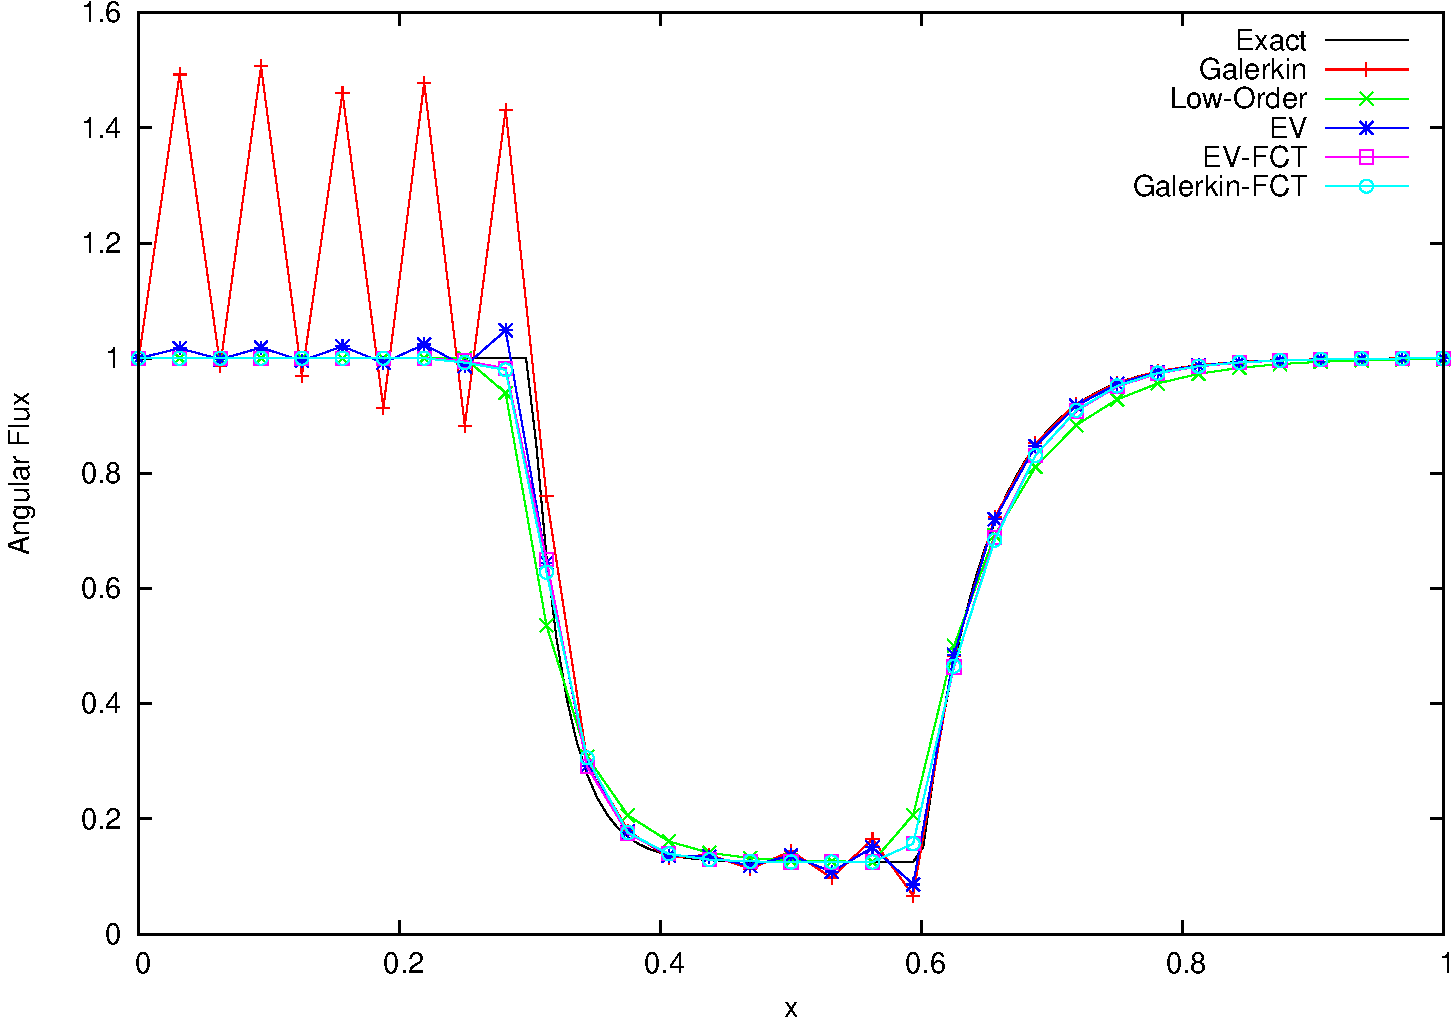
\includegraphics[width=0.9\textwidth]
     {\contentdir/results/transport/three_region/three_region.pdf}
   \caption{Comparison of Solutions for the 3-Region Test Problem Using SSPRK33 with 32 Cells}
   \label{fig:three_region}
\end{figure}
%-------------------------------------------------------------------------------

\clearpage
